\documentclass[a4paper,12pt]{article}
\usepackage[utf8]{inputenc}
\usepackage{graphicx}

\begin{document}

\section{Auswertung}

\begin{figure}
 \begin{center}
 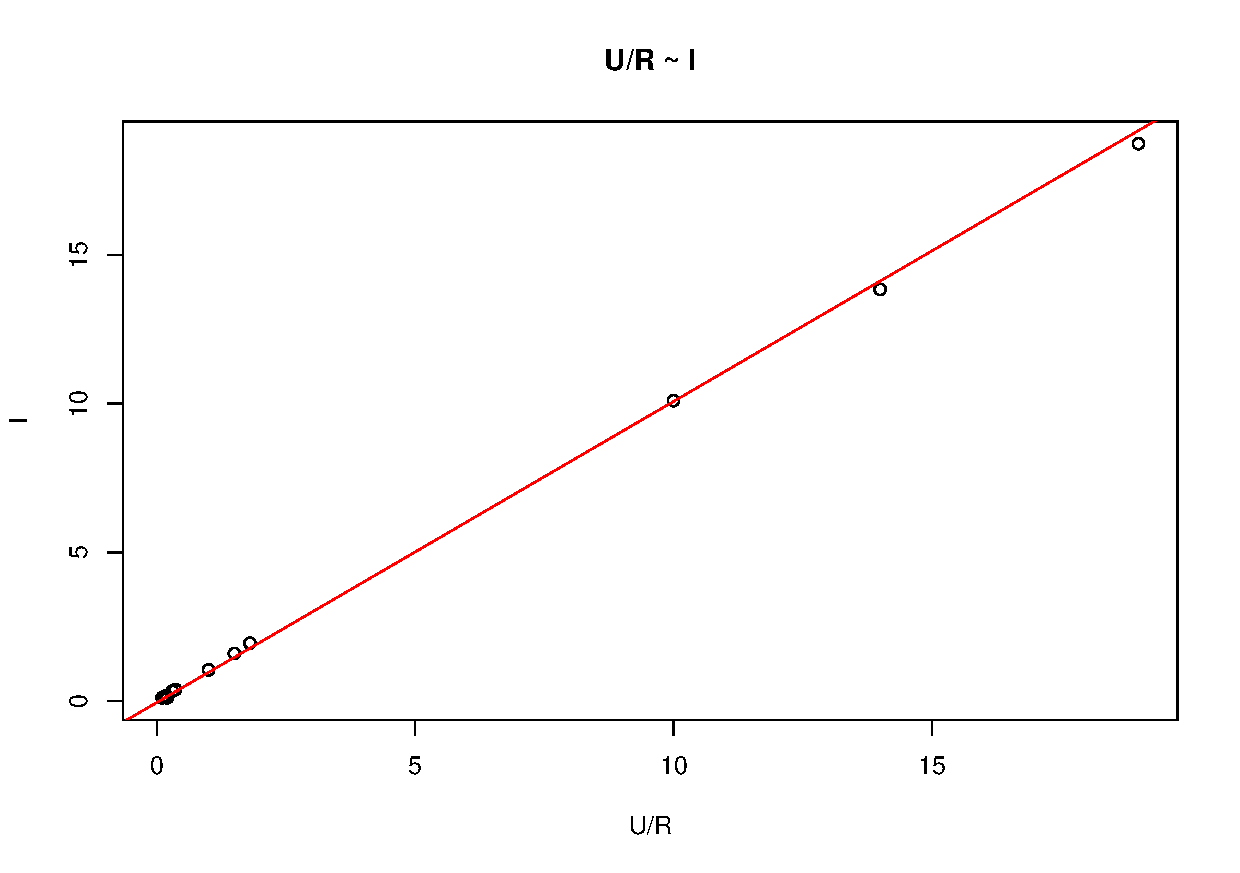
\includegraphics[scale=0.6]{R/plot.pdf}      
 \caption{Messwerte des ersten Versuchs}
 \label{fig:messwerte} 
 \end{center}
\end{figure}

Wie wir deutlich herausarbeiten konnten, ist das Ohmsche Gesetz gültig. Abbildung \ref{fig:messwerte} zeigt einen eindeutigen linearen Zusammenhang zwischen Spannung, Widerstand und Stromfluss. 

\section{Anhang}

\listoffigures

\end{document}





